W tym rozdziale przedstawiono wyniki procesu uczenia w środowisku Botbowl porównywanych sieci neuronowych. Celem przeprowadzonych eksperymentów było określenie wpływu architektury sieci neuronowej na zdolność agenta do nauki skutecznej polityki gry w środowisku o bardzo dużej przestrzeni stanów oraz wysokim współczynniku branching factor.

Środowisko Blood Bowl jest szczególnie wymagające z punktu widzenia uczenia ze wzmocnieniem. W wielu stanach gry agent ma do wyboru bardzo dużą liczbę możliwych akcji, a konsekwencje podjętych decyzji mogą ujawniać się dopiero po wielu kolejnych krokach. Powoduje to, że proces uczenia charakteryzuje się dużą wariancją, a stabilność algorytmu oraz zdolność modelu do ekstrakcji istotnych cech ze stanu gry odgrywają kluczową rolę.

\subsection*{Zastosowane miary jakości}
\label{sec:metryki}

W trakcie uczenia zbierane były 3 statystyki określające postęp uczenia.

Wykresy \textit{Win rate}, tj. odsetek zwycięstw w rozgrywkach ewaluacyjnych. Wartość około $0.5$ oznacza poziom zbliżony do przeciwnika (w przybliżeniu ``remis'' sił), natomiast wartości istotnie wyższe od $0.5$ wskazują na realną poprawę skuteczności agenta.

Wykres \textit{Reward} przedstawia średnią (lub uśrednianą w oknie) nagrodę uzyskiwaną przez agenta w trakcie treningu. Ponieważ w Blood Bowl nagrody są w dużej mierze rzadkie i silnie zależne od długoterminowych konsekwencji decyzji, sama wartość \textit{Reward} może charakteryzować się dużą wariancją i nie zawsze wprost przekłada się na poprawę jakości gry.

Wykres \textit{TD/Episode} raportuje liczbę przyłożeń na epizod osobno dla uczącego się agenta (\textit{Learner}) oraz przeciwnika (\textit{Opponent}). Miara ta jest bardziej bezpośrednio związana z przebiegiem meczu niż \textit{Reward}, jednak również bywa rzadka (w wielu partiach liczba przyłożeń jest niska), przez co pojawiają się skoki zamiast gładkich trendów.

Spośród przedstawionych miar najważniejszym wskaźnikiem jakości wyuczonej polityki jest \textit{Win rate}, ponieważ bezpośrednio odzwierciedla skuteczność agenta w rozgrywce przeciwko przeciwnikowi testowemu.

\subsection*{Wyniki}

Na poniższych wykresach przedstawiono porównanie wyników dla wszystkich analizowanych konfiguracji architektur sieci neuronowych. Wykresy prezentują zależność analizowanych metryk od liczby iteracji treningowych.

\begin{tabular}{l}
	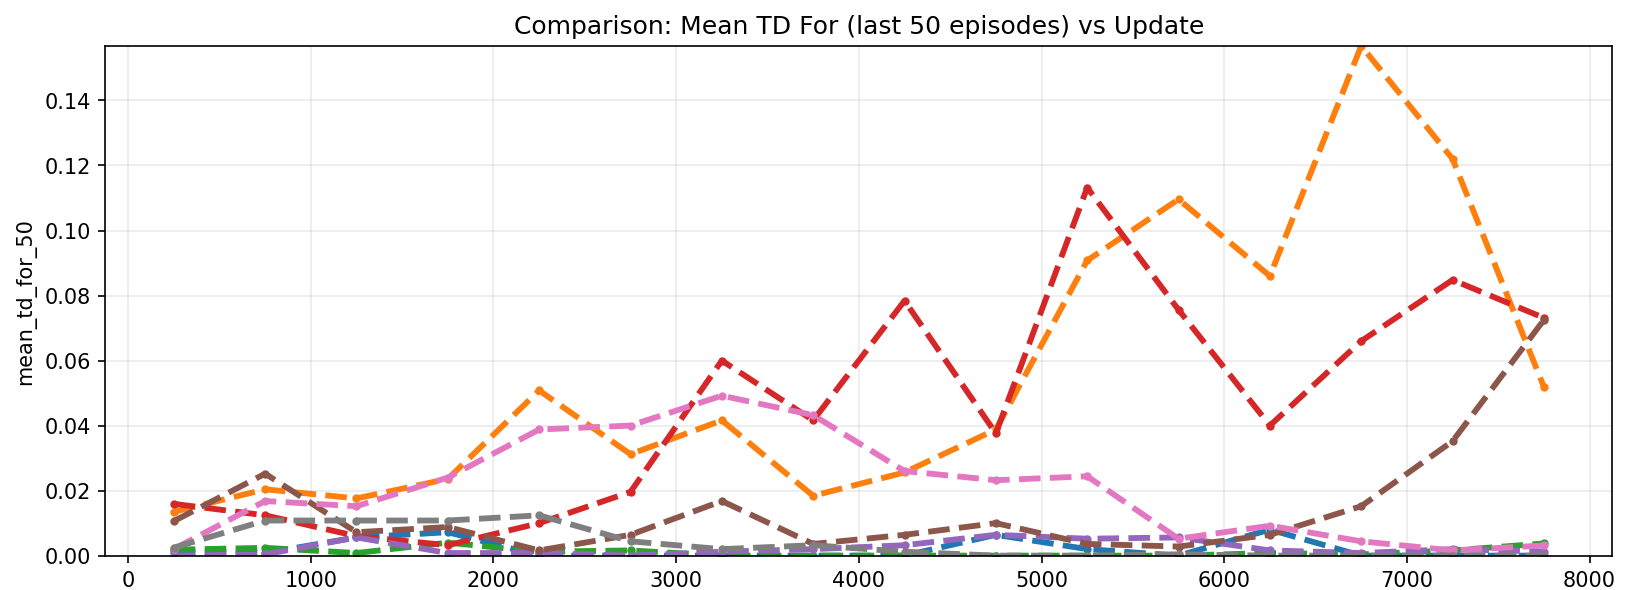
\includegraphics[width=\linewidth,height=6.2cm,keepaspectratio]{rysunki/compare_mean_td_for_50_no_legend.png}\\
	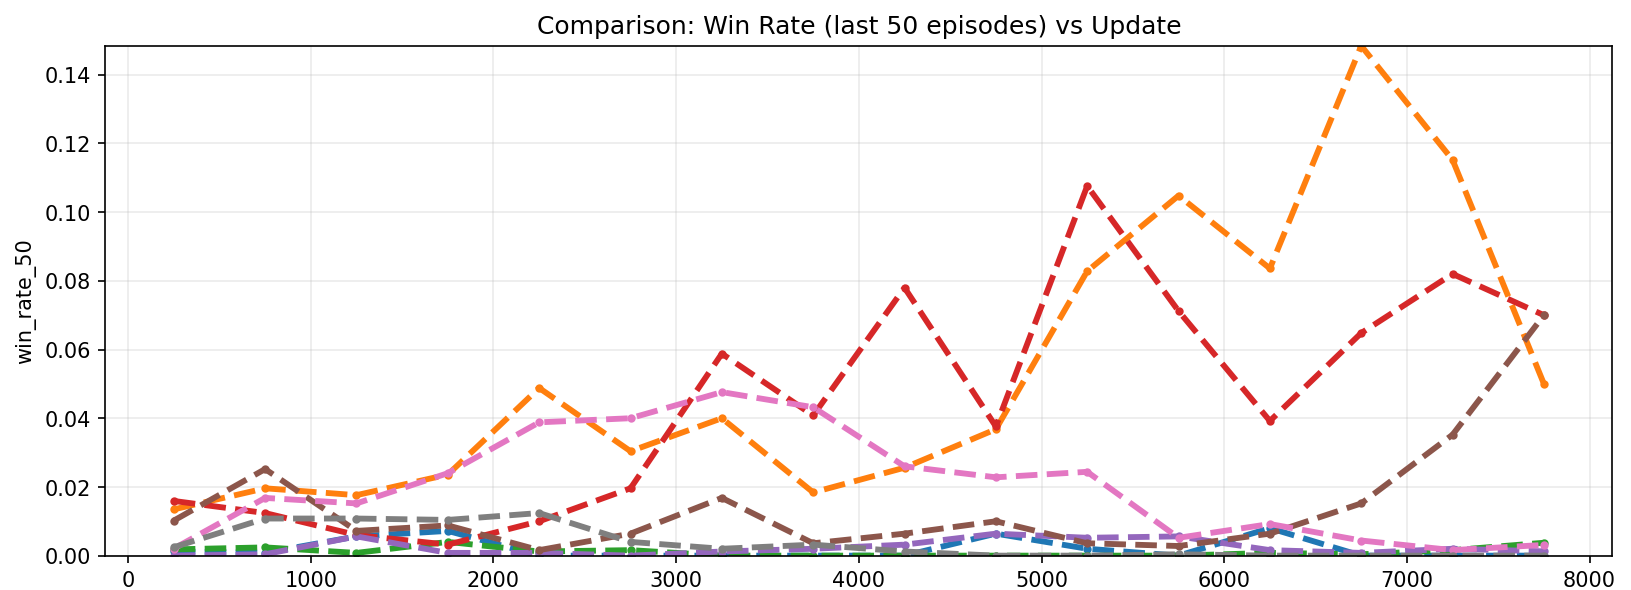
\includegraphics[width=\linewidth,height=6.2cm,keepaspectratio]{rysunki/compare_win_rate_50_no_legend.png}\\
	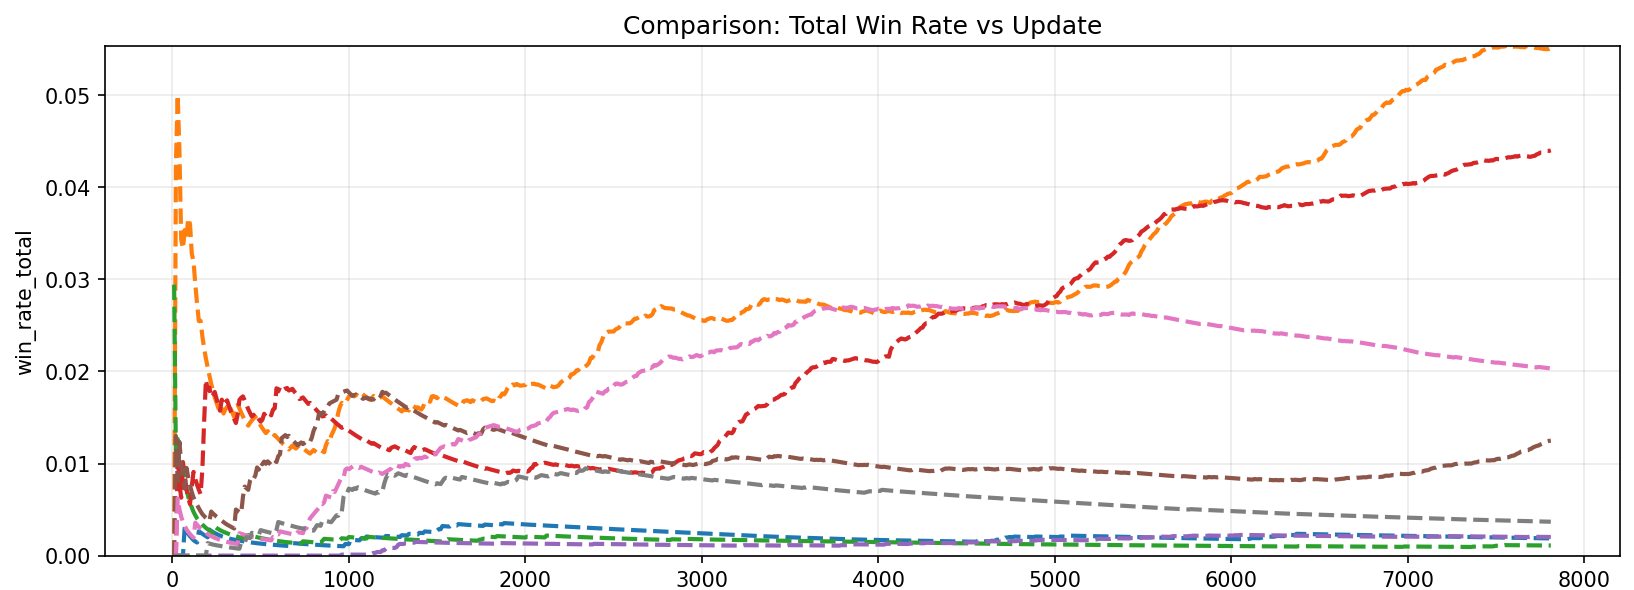
\includegraphics[width=\linewidth,height=6.2cm,keepaspectratio]{rysunki/compare_win_rate_total_no_legend.png}
\end{tabular}
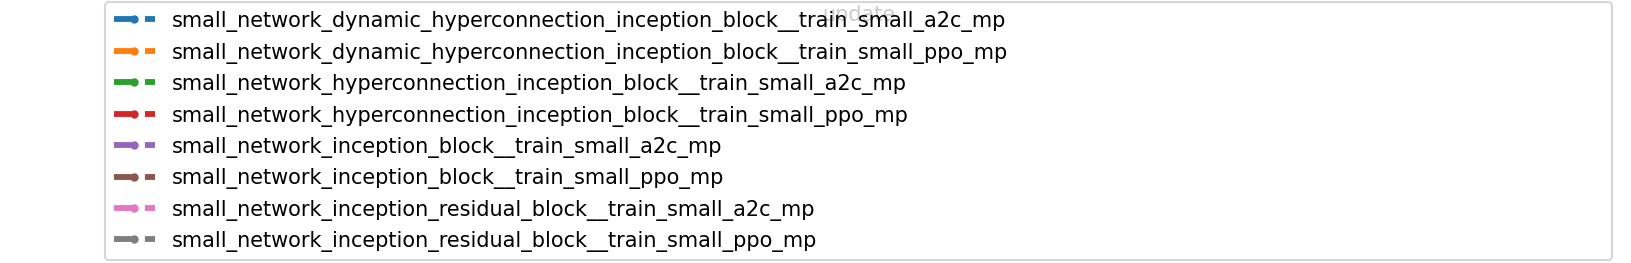
\includegraphics[width=\linewidth,height=6.2cm,keepaspectratio]{rysunki/legend.png}

Pierwszy z powyższych wykresów przedstawia średnią liczbę przyłożeń na epizod dla ostatnich 50 rozegranych epizodów. Wraz z postępem treningu można zaobserwować wzrost tej wartości dla części analizowanych konfiguracji, co wskazuje na stopniową poprawę zdolności agenta do skutecznego prowadzenia akcji ofensywnych.

Drugi wykres przedstawia średnią wartość wskaźnika \textit{Win rate} obliczaną w oknie obejmującym ostatnie 50 epizodów. Metryka ta pozwala obserwować krótkoterminowe zmiany jakości gry agenta w trakcie treningu. W przypadku części architektur widoczny jest systematyczny wzrost wartości tej miary, co wskazuje na stopniową poprawę wyuczonej polityki.

Trzeci wykres przedstawia całkowity wskaźnik zwycięstw w funkcji liczby iteracji treningowych. W przeciwieństwie do poprzedniego wykresu, miara ta ma charakter bardziej globalny i pokazuje długoterminowy trend skuteczności agenta. Wraz z postępem uczenia można zaobserwować stopniowy wzrost tej wartości dla najlepszych konfiguracji architektur.

\begin{tabular}{l}
	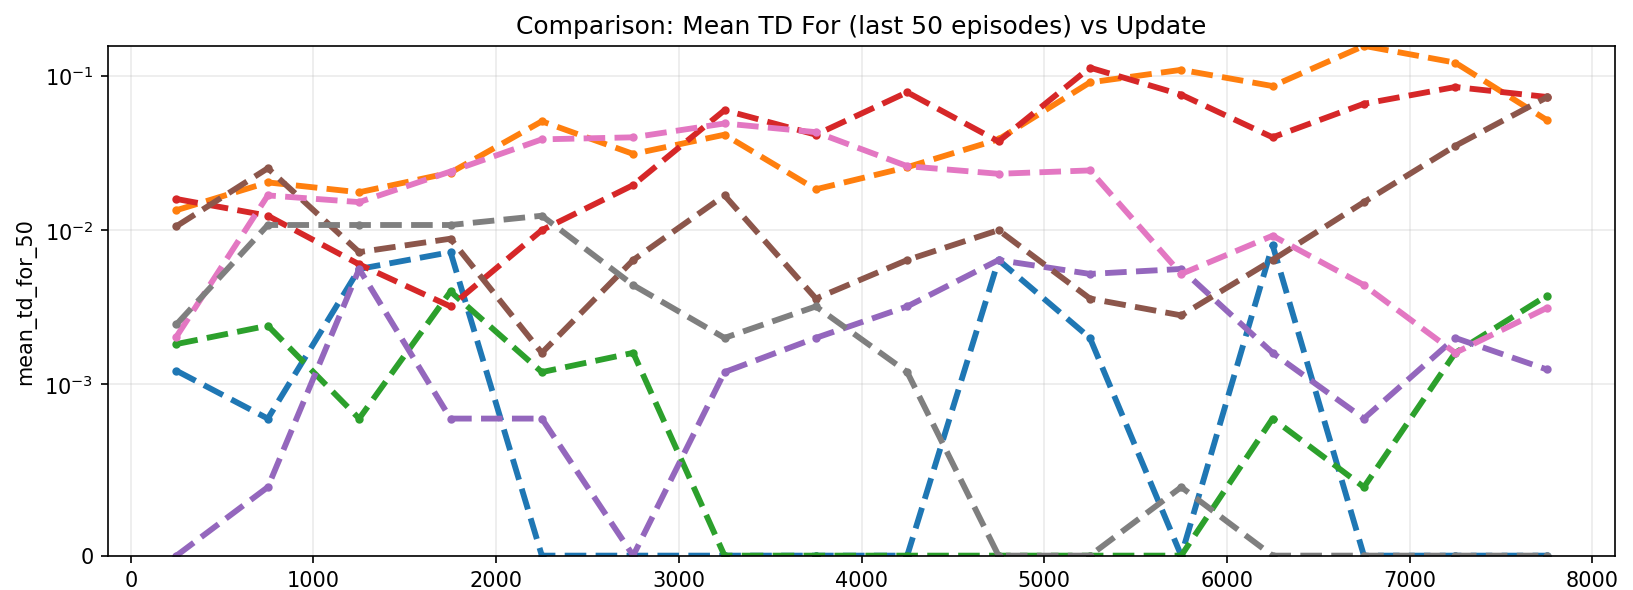
\includegraphics[width=\linewidth,height=6.2cm,keepaspectratio]{rysunki/compare_mean_td_for_50_log_no_legend.png}\\
	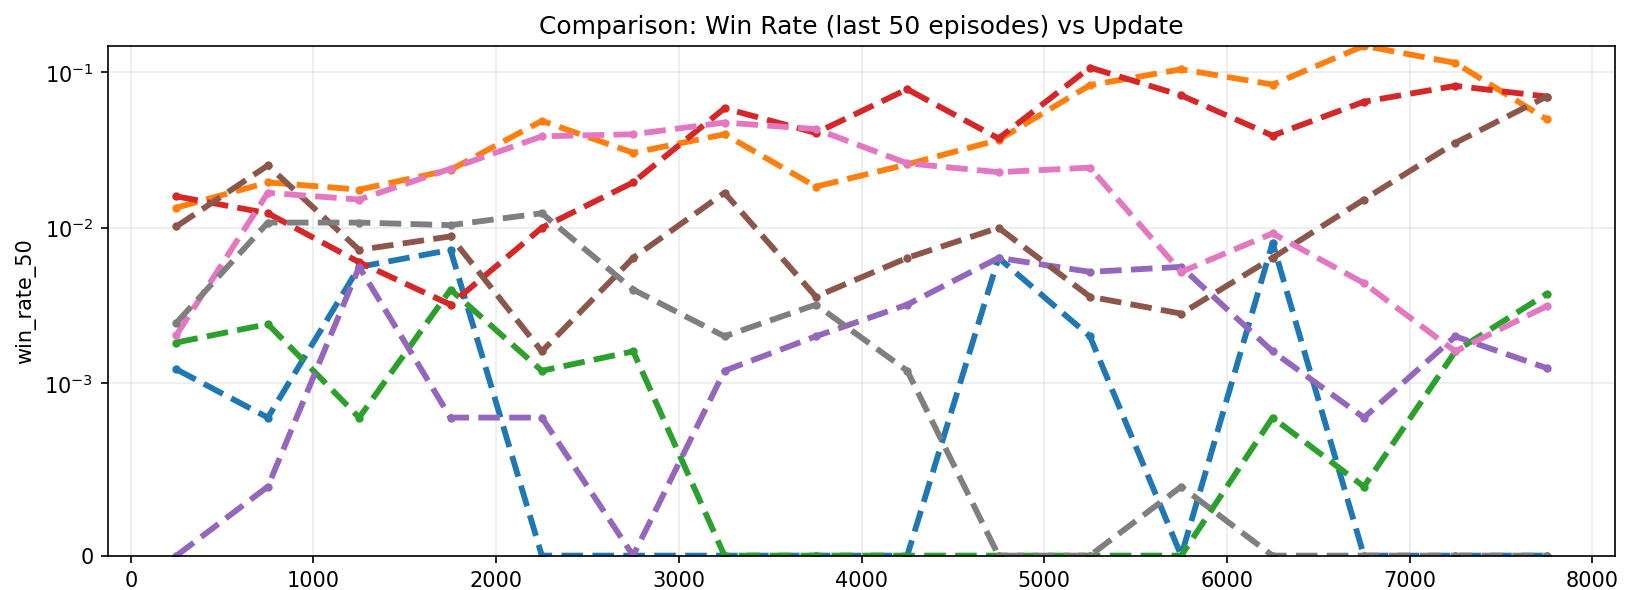
\includegraphics[width=\linewidth,height=6.2cm,keepaspectratio]{rysunki/compare_win_rate_50_log_no_legend.png}\\
	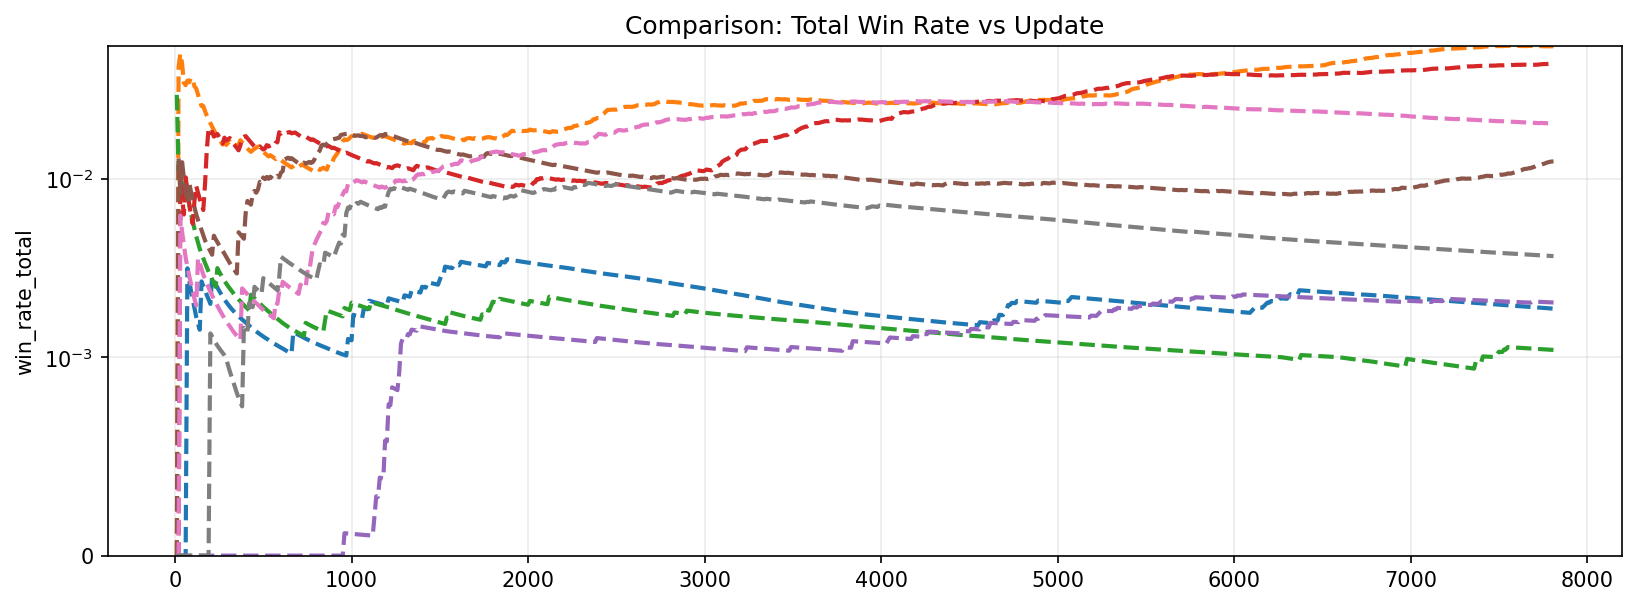
\includegraphics[width=\linewidth,height=6.2cm,keepaspectratio]{rysunki/compare_win_rate_total_log_no_legend.png}
\end{tabular}
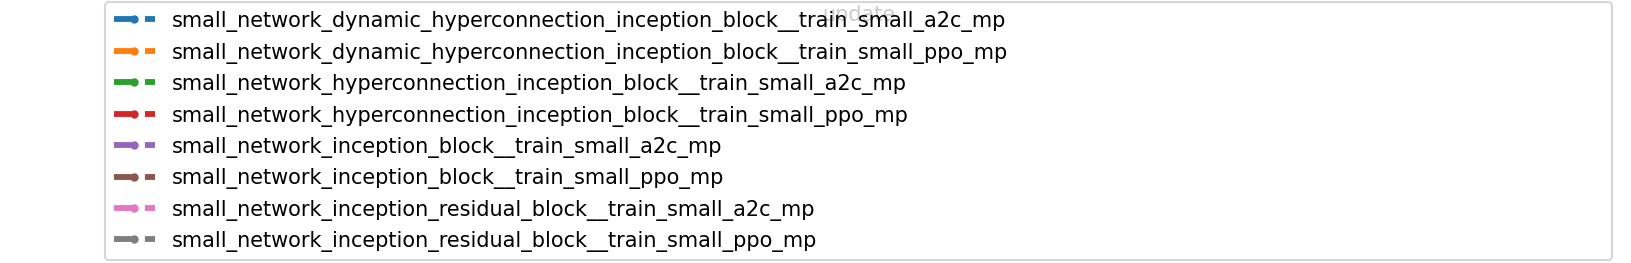
\includegraphics[width=\linewidth,height=6.2cm,keepaspectratio]{rysunki/legend.png}

Dodatkowo przedstawiono te same wykresy w skali logarytmicznej. Pozwala to lepiej uwidocznić różnice pomiędzy poszczególnymi konfiguracjami w początkowych etapach treningu, gdy wartości analizowanych metryk są jeszcze stosunkowo niewielkie.

Zastosowanie skali logarytmicznej umożliwia również łatwiejszą obserwację dynamiki wzrostu analizowanych wskaźników w kolejnych etapach procesu uczenia.



Legenda przedstawiona powyżej umożliwia identyfikację poszczególnych konfiguracji architektur analizowanych w eksperymentach.

\subsection*{Ograniczenia eksperymentu}

Należy zauważyć, że przeprowadzone eksperymenty posiadają pewne ograniczenia. Przede wszystkim liczba iteracji treningowych była ograniczona przez dostępne zasoby obliczeniowe, co mogło wpłynąć na możliwość pełnej konwergencji niektórych modeli.

Ponadto środowisko Blood Bowl charakteryzuje się znaczną losowością wynikającą z mechaniki gry, w szczególności z rzutów kośćmi. Powoduje to dużą wariancję uzyskiwanych wyników, co utrudnia jednoznaczną ocenę jakości wyuczonej polityki na podstawie pojedynczych przebiegów treningu.

Dodatkowo wszystkie eksperymenty zostały przeprowadzone przeciwko określonemu przeciwnikowi testowemu. W praktyce skuteczność wyuczonej strategii może zależeć od stylu gry przeciwnika, dlatego dalsze badania mogłyby obejmować ewaluację agentów przeciwko większej liczbie różnych strategii.

\subsection*{Wnioski}

Na podstawie przeprowadzonych eksperymentów można sformułować następujące wnioski:

\begin{itemize}
	
	\item Architektura sieci neuronowej ma istotny wpływ na zdolność agenta do nauki skutecznej polityki gry w środowisku Blood Bowl.
	
	\item W środowiskach o dużej przestrzeni stanów oraz wysokim branching factor szczególnie ważna jest zdolność modelu do efektywnej ekstrakcji cech opisujących stan gry.
	
	\item Analiza przebiegu metryk \textit{Win rate} oraz \textit{TD/Episode} wskazuje, że część architektur umożliwia stopniową poprawę jakości strategii agenta wraz z postępem treningu.
	
	\item Uzyskane wyniki wskazują również potencjalne kierunki dalszych badań, takie jak zastosowanie głębszych architektur konwolucyjnych, mechanizmów uwagi (attention) lub bardziej zaawansowanych algorytmów uczenia ze wzmocnieniem.
	
\end{itemize}






